\documentclass{article}

% content/resources/templates/preamble.tex
\usepackage[margin=0.6in]{geometry}
\author{Milav Dabgar}
\usepackage{amsmath,amssymb,amsthm}
\usepackage{booktabs}
\usepackage{multirow}
\usepackage{xcolor}
\usepackage{tcolorbox}
\tcbuselibrary{breakable,skins}
\usepackage[colorlinks=true,linkcolor=blue]{hyperref}
\usepackage{titlesec}
\usepackage{enumitem}
\usepackage{tikz}
\usepackage{pgfplots}
\usepackage{circuitikz}
\usepackage[version=4]{mhchem}
\usepackage{longtable}
\usepackage{array}
\usepackage{float}
\usepackage{caption}
\usepackage{listings}

\lstset{
  basicstyle=\small\ttfamily,
  breaklines=true,
  breakatwhitespace=false,
  postbreak=\mbox{\textcolor{red}{$\hookrightarrow$}\space},
  float=false,
  numbers=left,
  numberstyle=\tiny\color{gray},
  numbersep=10pt,
  xleftmargin=2em,
  keywordstyle=\color{blue},
  commentstyle=\color{green!60!black},
  stringstyle=\color{purple},
  backgroundcolor=\color{gray!5},
  showstringspaces=false,
  tabsize=2,
  captionpos=b,
  keepspaces=true,
  columns=flexible
}

\pgfplotsset{compat=1.18}
\usetikzlibrary{shapes,arrows,positioning,calc,patterns,decorations.pathmorphing,decorations.markings,arrows.meta}

% Color scheme
\definecolor{headcolor}{RGB}{0,102,204}
\definecolor{keycolor}{RGB}{220,20,60}
\definecolor{solutioncolor}{RGB}{34,139,34}
\definecolor{mnemoniccolor}{RGB}{148,0,211}
\definecolor{codecolor}{RGB}{0,0,100}

% Spacing
\setlength{\parskip}{3pt}
\setlist[itemize]{nosep}
\setlist[enumerate]{nosep}

% Title formatting
\titleformat{\section}{\Large\bfseries\color{headcolor}}{\thesection}{1em}{}
\titleformat{\subsection}{\large\bfseries\color{headcolor}}{\thesubsection}{1em}{}

% Pandoc tightlist compatibility
\providecommand{\tightlist}{%
  \setlength{\itemsep}{0pt}\setlength{\parskip}{0pt}}

% Pandoc longtable compatibility
\newcounter{none}
\def\thenone{}


% content/resources/templates/english-boxes.tex

% Custom environments
\newtcolorbox{solutionbox}{
 breakable,
 enhanced,
 colback=solutioncolor!5!white,
 colframe=solutioncolor!75!black,
 fonttitle=\bfseries,
 title=Solution
}

\newtcolorbox{solutionboxnobreak}{
 colback=solutioncolor!5!white,
 colframe=solutioncolor!75!black,
 fonttitle=\bfseries,
 title=Solution
}

\newtcolorbox{keyformula}{
 breakable,
 enhanced,
 colback=keycolor!5!white,
 colframe=keycolor!75!black,
 fonttitle=\bfseries,
 title=Key Formula
}

\newtcolorbox{mnemonicboxenv}{
 breakable,
 enhanced,
 colback=mnemoniccolor!5!white,
 colframe=mnemoniccolor!75!black,
 fonttitle=\bfseries,
 title=Mnemonic
}

\newcommand{\mnemonicbox}[1]{%
  \begin{mnemonicboxenv}
    #1
  \end{mnemonicboxenv}
}


% Custom commands for GTU solutions
% This file defines semantic commands for consistent formatting

% Question command with automatic formatting
\newcommand{\question}[2]{%
  \section*{Question #1}%
  \textbf{#2}%
}

% OR question variant
\newcommand{\questionor}[2]{%
  \section*{Question #1 OR}%
  \textbf{#2}%
}

% Proper table environment with caption
\newenvironment{answertable}[1]{%
  \begin{table}[htbp]
  \centering
  \caption{#1}
}{%
  \end{table}
}

% Proper figure environment for diagrams
\newenvironment{answerdiagram}[1]{%
  \begin{figure}[htbp]
  \centering
  \caption{#1}
}{%
  \end{figure}
}

% Semantic markup for key terms
\newcommand{\keyword}[1]{\textbf{#1}}
\newcommand{\code}[1]{\texttt{#1}}
\newcommand{\classname}[1]{\texttt{#1}}
\newcommand{\methodname}[1]{\texttt{#1}}

% Proper quotation marks
\newcommand{\mnemonic}[1]{``#1''}


\title{Electronic Circuits \& Networks (4331101) - Winter 2022 Solution}
\date{February 23, 2023}

\begin{document}
\maketitle

\section*{Question 1(a) [3 marks]}
\questionmarks{Question 1(a)}{3}{marks}

\textbf{Define: 1) Branch 2) Junction 3) Mesh}

\begin{solutionbox}
\begin{itemize}
    \item \textbf{Branch}: A branch is a single circuit element or a combination of elements connected between two nodes of a network.
    \item \textbf{Junction}: A junction (or node) is a point in a circuit where two or more circuit elements are connected together.
    \item \textbf{Mesh}: A mesh is a closed path in a network where no other closed path exists inside it.
\end{itemize}

\begin{mnemonicbox}
"BJM: Branches Join at junctions to Make meshes"
\end{mnemonicbox}
\end{solutionbox}

\section*{Question 1(b) [4 marks]}
\questionmarks{Question 1(b)}{4}{marks}

\textbf{Write voltage division and current division rule with necessary circuit diagram}

\begin{solutionbox}
\textbf{Voltage Division Rule}: In a series circuit, voltage across any component is proportional to its resistance.

\begin{center}
\begin{circuitikz}[american, scale=0.8]
    \draw (0,0) to[V, l=$V_S$, invert] (0,3)
          to[R, l=$R_1$, v=$V_1$] (3,3)
          to[R, l=$R_2$, v=$V_2$] (3,0) -- (0,0);
\end{circuitikz}
\captionof{figure}{Voltage Division Circuit}
\end{center}

\begin{itemize}
    \item \textbf{Formula}: $V_1 = V_S \times \frac{R_1}{R_1+R_2}$
    \item \textbf{Application}: Used to find individual voltage drops across series components
\end{itemize}

\textbf{Current Division Rule}: In a parallel circuit, current through any branch is inversely proportional to its resistance.

\begin{center}
\begin{circuitikz}[american, scale=0.8]
    \draw (0,0) to[I, l=$I_S$] (0,3) -- (4,3);
    \draw (2,3) to[R, l=$R_1$, i=$I_1$] (2,0);
    \draw (4,3) to[R, l=$R_2$, i=$I_2$] (4,0);
    \draw (0,0) -- (4,0);
\end{circuitikz}
\captionof{figure}{Current Division Circuit}
\end{center}

\begin{itemize}
    \item \textbf{Formula}: $I_1 = I_S \times \frac{R_2}{R_1+R_2}$
    \item \textbf{Key concept}: Current takes path of least resistance
\end{itemize}

\begin{mnemonicbox}
"VoSe CuPa: Voltage divides in Series, Current divides in Parallel"
\end{mnemonicbox}
\end{solutionbox}

\section*{Question 1(c) [7 marks]}
\questionmarks{Question 1(c)}{7}{marks}

\textbf{Draw Graph and Tree for a network shown in fig(1). Show link currents on a graph. Also write Tie-set schedule for a tree of network shown in fig. (1)}

\begin{solutionbox}
\textbf{Graph of the Network}:

\begin{center}
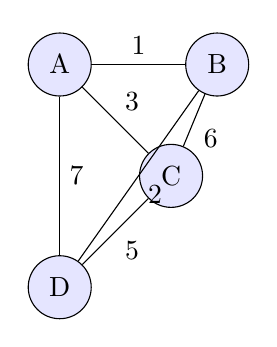
\begin{tikzpicture}[auto, node distance=2cm, main/.style={circle,draw,fill=blue!10,minimum size=0.8cm,inner sep=0pt}]
    \node[main] (A) {A};
    \node[main] (B) [right of=A] {B};
    \node[main] (C) [below right of=A] {C};
    \node[main] (D) [below left of=C] {D};

    \path[draw]
    (A) edge node {1} (B)
    (A) edge node {3} (C)
    (A) edge node {7} (D)
    (B) edge node {2} (D)
    (B) edge node {6} (C)
    (C) edge node {5} (D);
\end{tikzpicture}
\captionof{figure}{Graph of the Network}
\end{center}

\textbf{Tree of the Network} (Twigs in solid, Links in dashed):

\begin{center}
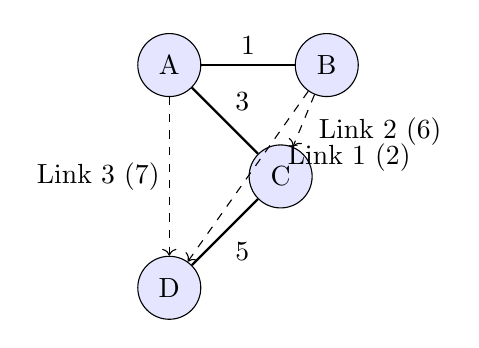
\begin{tikzpicture}[auto, node distance=2cm, main/.style={circle,draw,fill=blue!10,minimum size=0.8cm,inner sep=0pt}]
    \node[main] (A) {A};
    \node[main] (B) [right of=A] {B};
    \node[main] (C) [below right of=A] {C};
    \node[main] (D) [below left of=C] {D};

    % Tree branches (Twigs) - Solid
    \draw[thick] (A) -- node {1} (B);
    \draw[thick] (A) -- node {3} (C);
    \draw[thick] (C) -- node {5} (D);

    % Links - Dashed with Link Currents
    \draw[dashed, ->] (B) -- node[near start] {Link 1 (2)} (D);
    \draw[dashed, ->] (B) -- node[near start] {Link 2 (6)} (C);
    \draw[dashed, ->] (A) -- node[swap] {Link 3 (7)} (D);
\end{tikzpicture}
\captionof{figure}{Tree and Links}
\end{center}

\textbf{Tie-set Schedule}:

\begin{tabulary}{\linewidth}{@{}|L|C|C|C|C|C|C|C|@{}}
    \hline
    \textbf{Link/Tree Branch} & \textbf{Br 1 (AB)} & \textbf{Br 3 (AC)} & \textbf{Br 4 (CD)} & \textbf{Br 2 (BD)} & \textbf{Br 6 (BC)} & \textbf{Br 7 (AD)} & \textbf{Br 5 (CD)} \\
    \hline
    Link 1 (BD) & 1 & 0 & 0 & 1 & 0 & 0 & 0 \\
    \hline
    Link 2 (BC) & 1 & 1 & 0 & 0 & 1 & 0 & 0 \\
    \hline
    Link 3 (AD) & 0 & 0 & 1 & 0 & 0 & 1 & 0 \\
    \hline
    Link 4 (CD) & 0 & 0 & 1 & 0 & 0 & 0 & 1 \\
    \hline
\end{tabulary}

\begin{mnemonicbox}
"TGLT: Trees Generate Link-current Tie-sets"
\end{mnemonicbox}
\end{solutionbox}

\section*{Question 1(c) OR [7 marks]}
\questionmarks{Question 1(c) OR}{7}{marks}

\textbf{Draw Graph and Tree for a network shown in fig(1). Show branch voltages on tree. Also write cut-set schedule for a tree of network shown on fig.(1)}

\begin{solutionbox}
\textbf{Graph of the Network}: Same as above.

\textbf{Tree of the Network}:

\begin{center}
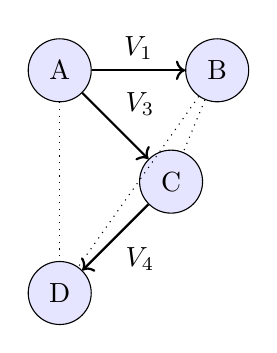
\begin{tikzpicture}[auto, node distance=2cm, main/.style={circle,draw,fill=blue!10,minimum size=0.8cm,inner sep=0pt}]
    \node[main] (A) {A};
    \node[main] (B) [right of=A] {B};
    \node[main] (C) [below right of=A] {C};
    \node[main] (D) [below left of=C] {D};

    % Tree branches with Voltages
    \draw[thick, ->] (A) -- node {$V_1$} (B);
    \draw[thick, ->] (A) -- node {$V_3$} (C);
    \draw[thick, ->] (C) -- node {$V_4$} (D);
    
    % Links just to show context, ghosted
    \draw[dotted] (B) -- (D);
    \draw[dotted] (B) -- (C);
    \draw[dotted] (A) -- (D);
\end{tikzpicture}
\captionof{figure}{Tree with Branch Voltages}
\end{center}

\textbf{Cut-set Schedule}:

\begin{tabulary}{\linewidth}{@{}|L|C|C|C|C|C|C|C|@{}}
    \hline
    \textbf{Cut-set/Branch} & \textbf{Br 1 (AB)} & \textbf{Br 3 (AC)} & \textbf{Br 4 (CD)} & \textbf{Br 2 (BD)} & \textbf{Br 6 (BC)} & \textbf{Br 7 (AD)} & \textbf{Br 5 (CD)} \\
    \hline
    Cut-set 1 (AB) & 1 & 0 & 0 & -1 & -1 & 0 & 0 \\
    \hline
    Cut-set 2 (AC) & 0 & 1 & 0 & 0 & 1 & -1 & 0 \\
    \hline
    Cut-set 3 (CD) & 0 & 0 & 1 & 1 & 0 & 1 & 1 \\
    \hline
\end{tabulary}

\begin{mnemonicbox}
"CGVS: Cut-sets Generate Voltage Sources"
\end{mnemonicbox}
\end{solutionbox}

\section*{Question 2(a) [3 marks]}
\questionmarks{Question 2(a)}{3}{marks}

\textbf{Define: 1) Active and passive network 2)Unilateral and Bilateral network.}

\begin{solutionbox}
\begin{itemize}
    \item \textbf{Active Network}: A network containing one or more sources of EMF (voltage/current sources) that supply energy to the circuit.
    \item \textbf{Passive Network}: A network containing only passive elements like resistors, capacitors, and inductors with no energy sources.
    
    \item \textbf{Unilateral Network}: A network in which the properties and performance change when input and output terminals are interchanged (e.g., diode circuits).
    \item \textbf{Bilateral Network}: A network in which the properties and performance remain unchanged when input and output terminals are interchanged (e.g., resistor circuits).
\end{itemize}

\begin{center}
\begin{tikzpicture}[gtu tree]
    \node [gtu root] {Network Types}
        child { node [gtu child] {Active\\(Contains Sources)} }
        child { node [gtu child] {Passive\\(No Sources)} }
        child { node [gtu child] {Unilateral\\(Diodes/Transistors)} }
        child { node [gtu child] {Bilateral\\(R, L, C elements)} };
\end{tikzpicture}
\captionof{figure}{Network Classification}
\end{center}

\begin{mnemonicbox}
"APUB: Active Provides energy, Unilateral Blocks reversal"
\end{mnemonicbox}
\end{solutionbox}

\section*{Question 2(b) [4 marks]}
\questionmarks{Question 2(b)}{4}{marks}

\textbf{Write equation for Z parameter and derive Z11, Z12, Z21, Z22 from that equation.}

\begin{solutionbox}
Z-parameters define the relationship between port voltages and currents in a two-port network:

\textbf{Equations}:
\begin{align*}
    V_1 &= Z_{11}I_1 + Z_{12}I_2 \\
    V_2 &= Z_{21}I_1 + Z_{22}I_2
\end{align*}

\textbf{Derivation}:
\begin{itemize}
    \item \textbf{$Z_{11} = \frac{V_1}{I_1} \bigg|_{I_2=0}$}: Input impedance with output port open-circuited.
    \item \textbf{$Z_{12} = \frac{V_1}{I_2} \bigg|_{I_1=0}$}: Reverse transfer impedance with input port open-circuited.
    \item \textbf{$Z_{21} = \frac{V_2}{I_1} \bigg|_{I_2=0}$}: Forward transfer impedance with output port open-circuited.
    \item \textbf{$Z_{22} = \frac{V_2}{I_2} \bigg|_{I_1=0}$}: Output impedance with input port open-circuited.
\end{itemize}

\begin{mnemonicbox}
"Z Impedance: Open circuit gives correct Parameters"
\end{mnemonicbox}
\end{solutionbox}

\section*{Question 2(c) [7 marks]}
\questionmarks{Question 2(c)}{7}{marks}

\textbf{Derive equation of characteristic impedance(ZOT) for a standard T network.}

\begin{solutionbox}
For a standard T-network:

\begin{center}
\begin{circuitikz}[american, scale=0.9]
    \draw (0,2) to[short, o-] (1,2) to[generic, l=$Z_1$] (3,2) coordinate(C) to[generic, l=$Z_2$] (5,2) to[short, -o] (6,2);
    \draw (C) to[generic, l=$Z_3$] (3,0) -- (3,0) coordinate(G);
    \draw (0,0) to[short, o-] (6,0) to[short, -o] (6,0);
    \node at (0,1) {Port 1};
    \node at (6,1) {Port 2};
\end{circuitikz}
\captionof{figure}{T-Network}
\end{center}

\textbf{Derivation Steps}:
\begin{enumerate}
    \item For a symmetric T-network, $Z_1 = Z_2$.
    \item Under matched condition, input impedance equals characteristic impedance.
    \item $Z_{0T} = Z_1 + \frac{Z_1 \times Z_3}{Z_1 + Z_3}$
    \item For balanced T-network where series arms are $Z/2$ and shunt arm is $Z$:
    \item $Z_{0T} = \frac{Z}{2} + \frac{\frac{Z}{2} \times Z}{\frac{Z}{2} + Z}$
    \item $Z_{0T} = \frac{Z}{2} + \frac{Z^2/2}{3Z/2}$
    \item $Z_{0T} = \frac{Z}{2} + \frac{Z}{3}$
    \item $Z_{0T} = \frac{3Z + 2Z}{6}$
    \item $Z_{0T} = \sqrt{Z_1(Z_1 + 2Z_3)}$
\end{enumerate}

\textbf{Final Equation}: $Z_{0T} = \sqrt{Z_1(Z_1 + 2Z_3)}$

\begin{mnemonicbox}
"TO Impedance: Two arms Over middle branch"
\end{mnemonicbox}
\end{solutionbox}

\section*{Question 2(a) OR [3 marks]}
\questionmarks{Question 2(a) OR}{3}{marks}

\textbf{Define: 1)Driving point impedance 2) Transfer impedance}

\begin{solutionbox}
\begin{itemize}
    \item \textbf{Driving Point Impedance}: The ratio of voltage to current at the same port/pair of terminals when all other independent sources are set to zero ($Z_{11} = V_1/I_1$).
    \item \textbf{Transfer Impedance}: The ratio of voltage at one port to the current at another port when all other independent sources are set to zero ($Z_{21} = V_2/I_1$).
\end{itemize}

\begin{center}
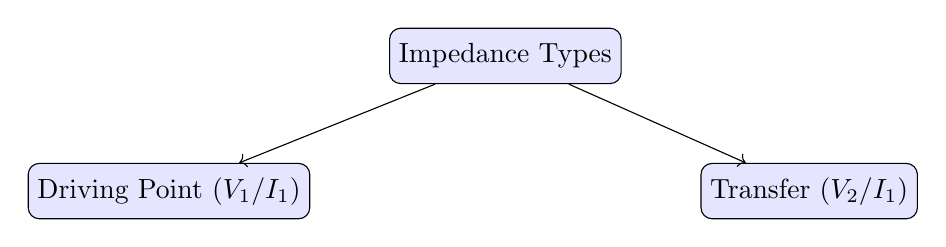
\begin{tikzpicture}[gtu block/.style={rectangle, draw, fill=blue!10, rounded corners, minimum height=2em}]
    \node[gtu block] (A) {Impedance Types};
    \node[gtu block] (B) [below left=of A] {Driving Point ($V_1/I_1$)};
    \node[gtu block] (C) [below right=of A] {Transfer ($V_2/I_1$)};
    \draw[->] (A) -- (B);
    \draw[->] (A) -- (C);
\end{tikzpicture}
\end{center}

\begin{mnemonicbox}
"DTSS: Driving at Terminal Same, Transfer at Separate"
\end{mnemonicbox}
\end{solutionbox}

\section*{Question 2(b) OR [4 marks]}
\questionmarks{Question 2(b) OR}{4}{marks}

\textbf{Explain Kirchhoff's voltage law with example.}

\begin{solutionbox}
\textbf{Kirchhoff's Voltage Law (KVL)}: The algebraic sum of all voltages around any closed loop in a circuit is zero.

\textbf{Mathematically}: $\sum V = 0$ (around a closed loop)

\textbf{Circuit Example}:

\begin{center}
\begin{circuitikz}[american, scale=0.8]
    \draw (0,0) to[V, l=10V, invert] (0,3)
          to[R, l={$R_1=2\Omega$}] (3,3)
          to[R, l={$R_2=3\Omega$}] (3,0)
          to[R, l={$R_3=5\Omega$}] (0,0);
\end{circuitikz}
\captionof{figure}{KVL Example Circuit}
\end{center}

If $I = 1A$, then:
\begin{itemize}
    \item $V_1 = 1A \times 2\Omega = 2V$
    \item $V_2 = 1A \times 3\Omega = 3V$
    \item $V_3 = 1A \times 5\Omega = 5V$
\end{itemize}

Applying KVL: $10V - 2V - 3V - 5V = 0$ \checkmark

\begin{mnemonicbox}
"VACZ: Voltages Around Closed loop are Zero"
\end{mnemonicbox}
\end{solutionbox}

\section*{Question 2(c) OR [7 marks]}
\questionmarks{Question 2(c) OR}{7}{marks}

\textbf{Derive equation to convert $\pi$ network into T network.}

\begin{solutionbox}
\textbf{$\pi$ Network to T Network Conversion}:

\begin{center}
\begin{circuitikz}[american, scale=0.8]
    % Pi Network
    \draw (0,2) to[short, o-] (1,2) to[short] (1,3) to[generic, l=$Y_a$] (4,3) to[short] (4,2) to[short, -o] (5,2);
    \draw (1,2) to[generic, l=$Y_c$] (1,0);
    \draw (4,2) to[generic, l=$Y_b$] (4,0);
    \draw (0,0) to[short, o-] (5,0) to[short, -o] (5,0);
    \node at (2.5, -1) {$\pi$ Network};
    
    % Arrow
    \draw[->, thick] (6, 1.5) -- (8, 1.5);
    
    % T Network
    \draw (9,2) to[short, o-] (10,2) to[generic, l=$Z_a$] (12,2) coordinate(C) to[generic, l=$Z_b$] (14,2) to[short, -o] (15,2);
    \draw (C) to[generic, l=$Z_c$] (12,0) -- (12,0);
    \draw (9,0) to[short, o-] (15,0) to[short, -o] (15,0);
    \node at (12, -1) {T Network};
\end{circuitikz}
\captionof{figure}{Conversion Diagram}
\end{center}

\textbf{Conversion Equations}:
\begin{itemize}
    \item $Z_a = \frac{Y_a \times Y_c}{Y_\Delta}$
    \item $Z_b = \frac{Y_b \times Y_c}{Y_\Delta}$
    \item $Z_c = \frac{Y_a \times Y_b}{Y_\Delta}$
\end{itemize}
Where $Y_\Delta = Y_a + Y_b + Y_c$

\textbf{Derivation}:
\begin{enumerate}
    \item Start with Y-parameters of $\pi$-network
    \item Express Y-parameters in terms of branch admittances
    \item Convert to Z-parameters using matrix inversion
    \item Express T-network impedances in terms of Z-parameters
    \item Simplify to get the conversion formulas above
\end{enumerate}

\begin{mnemonicbox}
"PIE to TEA: Product over sum for opposite branch"
\end{mnemonicbox}
\end{solutionbox}

\section*{Question 3(a) [3 marks]}
\questionmarks{Question 3(a)}{3}{marks}

\textbf{Explain Kirchhoff's current law with example.}

\begin{solutionbox}
\textbf{Kirchhoff's Current Law (KCL)}: The algebraic sum of all currents entering and leaving a node must equal zero.

\textbf{Mathematically}: $\sum I = 0$ (at any node)

\textbf{Circuit Example}:
\begin{center}
\begin{circuitikz}[american, scale=0.8]
    \node[circ] (B) at (2,2) {};
    \draw (0,4) to[short, i=$I_1=5A$] (B);
    \draw (0,0) to[short, i=$I_2=2A$] (B);
    \draw (B) to[short, i=$I_3=3A$] (4,4);
    \draw (B) to[short, i=$I_4=4A$] (4,0);
    \node[above] at (B) {Node B};
\end{circuitikz}
\end{center}

Applying KCL at node B:
\begin{itemize}
    \item Currents entering: $I_1 + I_2 = 5A + 2A = 7A$
    \item Currents leaving: $I_3 + I_4 = 3A + 4A = 7A$
    \item Therefore: $I_1 + I_2 - I_3 - I_4 = 5 + 2 - 3 - 4 = 0$ \checkmark
\end{itemize}

\begin{mnemonicbox}
"CuNoZ: Currents at Node are Zero"
\end{mnemonicbox}
\end{solutionbox}

\section*{Question 3(b) [4 marks]}
\questionmarks{Question 3(b)}{4}{marks}

\textbf{Explain mesh analysis with required equations.}

\begin{solutionbox}
\textbf{Mesh Analysis}: A circuit analysis technique that uses mesh currents as variables to solve a circuit with multiple loops.

\textbf{Steps}:
\begin{enumerate}
    \item Identify all meshes (closed loops) in the circuit
    \item Assign a mesh current to each mesh
    \item Apply KVL to each mesh
    \item Solve the resulting system of equations
\end{enumerate}

\textbf{Example Circuit}:
\begin{center}
\begin{circuitikz}[american, scale=0.8]
    \draw (0,0) to[V, l=$V_1$, invert] (0,3)
          to[R, l=$R_1$] (3,3)
          to[R, l=$R_2$] (3,0) -- (0,0);
    \draw (3,3) to[R, l=$R_3$] (6,3)
          to[V, l=$V_2$] (6,0) -- (3,0);
    \draw[->] (1.5,1.5) arc (-60:240:0.5) node[midway, below] {$I_1$};
    \draw[->] (4.5,1.5) arc (-60:240:0.5) node[midway, below] {$I_2$};
\end{circuitikz}
\captionof{figure}{Mesh Analysis Example}
\end{center}

\textbf{Equations}:
\begin{itemize}
    \item Mesh 1: $V_1 = I_1R_1 + (I_1-I_2)R_2$
    \item Mesh 2: $V_2 = I_2R_3 + (I_2-I_1)R_2$
\end{itemize}

\begin{mnemonicbox}
"MILK: Mesh Is Loop with KVL"
\end{mnemonicbox}
\end{solutionbox}

\section*{Question 3(c) [7 marks]}
\questionmarks{Question 3(c)}{7}{marks}

\textbf{State and explain Thevenin's theorem.}

\begin{solutionbox}
\textbf{Thevenin's Theorem}: Any linear network with voltage and current sources can be replaced by an equivalent circuit consisting of a voltage source ($V_{TH}$) in series with a resistance ($R_{TH}$).

\begin{center}
\begin{circuitikz}[american]
    \draw (0,0) node[circ, label=left:B]{} to[short] (1,0) to[R, l=$R_{TH}$] (3,0) to[V, l=$V_{TH}$] (3,2) to[short] (0,2) node[circ, label=left:A]{};
    \draw (4,1) node{\Huge $\equiv$};
    \draw (5,0) node[draw, minimum width=2cm, minimum height=2cm] (box) {Linear Network};
    \node at (4.5, 2) {Original};
    \node at (1.5, 2.5) {Equivalent};
\end{circuitikz}
\captionof{figure}{Thevenin Equivalent}
\end{center}

\textbf{Steps to Find Thevenin Equivalent}:
\begin{enumerate}
    \item Remove the load from the terminals of interest
    \item Calculate the open-circuit voltage ($V_{OC}$) across these terminals (= $V_{TH}$)
    \item Calculate the resistance looking back into the circuit with all sources replaced by their internal resistances (= $R_{TH}$)
    \item The Thevenin equivalent consists of $V_{TH}$ in series with $R_{TH}$
\end{enumerate}

\begin{mnemonicbox}
"TORV: Thevenin's Open-circuit Resistance and Voltage"
\end{mnemonicbox}
\end{solutionbox}

\section*{Question 3(a) OR [3 marks]}
\questionmarks{Question 3(a) OR}{3}{marks}

\textbf{State and explain reciprocity theorem.}

\begin{solutionbox}
\textbf{Reciprocity Theorem}: In a linear, bilateral network, if a voltage source in one branch produces a current in another branch, then the same voltage source, if placed in the second branch, will produce the same current in the first branch.

\begin{center}
\begin{circuitikz}[american, scale=0.8]
    % Case 1
    \draw (0,0) to[V, l=$V$] (0,2) -- (1,2) to[twoport, t=Network] (3,2) -- (4,2) to[rmeter, t=A] (4,0) -- (0,0);
    \node at (2,-0.5) {Original};
    
    % Case 2
    \draw (6,0) to[rmeter, t=A] (6,2) -- (7,2) to[twoport, t=Network] (9,2) -- (10,2) to[V, l=$V$] (10,0) -- (6,0);
    \node at (8,-0.5) {Reciprocal};
\end{circuitikz}
\end{center}

\textbf{Mathematically}: If a voltage $V_1$ in branch 1 produces current $I_2$ in branch 2, then voltage $V_1$ in branch 2 will produce current $I_2$ in branch 1.

\textbf{Limitations}: Applies only to networks with:
\begin{itemize}
    \item Linear elements
    \item Bilateral elements (no diodes, transistors)
    \item Single independent source
\end{itemize}

\begin{mnemonicbox}
"RESWAP: REciprocity SWAPs Position with identical results"
\end{mnemonicbox}
\end{solutionbox}

\section*{Question 3(b) OR [4 marks]}
\questionmarks{Question 3(b) OR}{4}{marks}

\textbf{Explain nodal analysis with required equations.}

\begin{solutionbox}
\textbf{Nodal Analysis}: A circuit analysis technique that uses node voltages as variables to solve a circuit.

\textbf{Steps}:
\begin{enumerate}
    \item Choose a reference node (ground)
    \item Assign voltage variables to remaining nodes
    \item Apply KCL at each non-reference node
    \item Solve the resulting system of equations
\end{enumerate}

\textbf{Example Circuit}:
\begin{center}
\begin{circuitikz}[american, scale=0.8]
    \draw (0,0) node[ground]{} to[I, l=$I_1$, invert] (0,3) node[circ, label=Node 1]{} 
          to[R, l=$G_3$] (4,3) node[circ, label=Node 2]{}
          to[I, l=$I_2$] (4,0) node[ground]{};
    \draw (0,3) to[R, l=$G_1$] (0,0);
    \draw (4,3) to[R, l=$G_2$] (4,0);
\end{circuitikz}
\captionof{figure}{Nodal Analysis}
\end{center}

\textbf{Equations}:
\begin{itemize}
    \item Node 1: $I_1 = V_1G_1 + (V_1-V_2)G_3$
    \item Node 2: $I_2 = V_2G_2 + (V_2-V_1)G_3$
\end{itemize}

\begin{mnemonicbox}
"NKCV: Nodal uses KCL with Voltage variables"
\end{mnemonicbox}
\end{solutionbox}

\section*{Question 3(c) OR [7 marks]}
\questionmarks{Question 3(c) OR}{7}{marks}

\textbf{State and prove maximum power transfer theorem.}

\begin{solutionbox}
\textbf{Maximum Power Transfer Theorem}: A load connected to a source will extract maximum power when its resistance equals the internal resistance of the source.

\begin{center}
\begin{circuitikz}[american]
    \draw (0,0) to[V, l=$V_S$] (0,3) to[R, l=$R_S$] (3,3) 
          to[R, l=$R_L$] (3,0) -- (0,0);
\end{circuitikz}
\end{center}

\textbf{Proof}:
\begin{enumerate}
    \item Current in the circuit: $I = \frac{V_S}{R_S + R_L}$
    \item Power delivered to load: $P = I^2R_L = \frac{V_S^2R_L}{(R_S + R_L)^2}$
    \item For maximum power, $\frac{dP}{dR_L} = 0$
    \item Solving: $\frac{V_S^2(R_S + R_L)^2 - V_S^2R_L \cdot 2(R_S + R_L)}{(R_S + R_L)^4} = 0$
    \item Simplifying: $(R_S + R_L)^2 = 2R_L(R_S + R_L)$
    \item Further simplifying: $R_S + R_L = 2R_L$
    \item Therefore: $R_S = R_L$
\end{enumerate}

\textbf{Maximum Power}: $P_{max} = \frac{V_S^2}{4R_S}$

\begin{mnemonicbox}
"MaRLRS: Maximum power when load Resistance equals Source Resistance"
\end{mnemonicbox}
\end{solutionbox}

\section*{Question 4(a) [3 marks]}
\questionmarks{Question 4(a)}{3}{marks}

\textbf{Why series resonance circuit act as voltage amplifier and parallel resonance circuit act as current amplifier?}

\begin{solutionbox}
\textbf{Series Resonance as Voltage Amplifier}:
\begin{itemize}
    \item At resonance, series circuit impedance is minimum (just R)
    \item Voltage across L or C can be much larger than source voltage
    \item Voltage magnification factor = $Q = \frac{X_L}{R} = \frac{1}{R}\sqrt{\frac{L}{C}}$
    \item Voltage across L or C = $Q \times$ Source voltage
\end{itemize}

\textbf{Parallel Resonance as Current Amplifier}:
\begin{itemize}
    \item At resonance, parallel circuit impedance is maximum
    \item Current in L or C can be much larger than source current
    \item Current magnification factor = $Q = \frac{R}{X_L} = R\sqrt{\frac{C}{L}}$
    \item Current through L or C = $Q \times$ Source current
\end{itemize}

\textbf{Table}:
\begin{tabulary}{\linewidth}{@{}|L|L|L|@{}}
    \hline
    \textbf{Circuit Type} & \textbf{Impedance at Resonance} & \textbf{Amplification} \\
    \hline
    Series & Minimum ($R$ only) & Voltage ($V_L$ or $V_C = Q \times V_S$) \\
    \hline
    Parallel & Maximum ($R^2/r$) & Current ($I_L$ or $I_C = Q \times I_S$) \\
    \hline
\end{tabulary}

\begin{mnemonicbox}
"SeVoPa: Series Voltage, Parallel current amplification"
\end{mnemonicbox}
\end{solutionbox}

\section*{Question 4(b) [4 marks]}
\questionmarks{Question 4(b)}{4}{marks}

\textbf{Derive equation of Q of coil.}

\begin{solutionbox}
\textbf{Q-factor of a Coil}:

\begin{center}
\begin{circuitikz}[american]
    \draw (0,0) to[R, l=$R$, o-o] (2,0) to[L, l=$L$, o-o] (4,0);
\end{circuitikz}
\end{center}

\textbf{Derivation}:
\begin{enumerate}
    \item Q-factor is defined as: $Q = \frac{\text{Energy stored}}{\text{Energy dissipated per cycle}}$
    \item Energy stored in inductor = $\frac{1}{2}LI^2$
    \item Power dissipated in resistor = $I^2R$
    \item Energy dissipated per cycle = Power $\times$ Time period = $I^2R \times \frac{1}{f}$
    \item Therefore: $Q = \frac{\frac{1}{2}LI^2}{I^2R \times \frac{1}{f}}$
    \item Simplifying: $Q = \frac{2\pi \times \frac{1}{2}LI^2 \times f}{I^2R}$
    \item $Q = \frac{2\pi f \times L}{R} = \frac{\omega L}{R}$
\end{enumerate}

\textbf{Final Equation}: $Q = \frac{\omega L}{R} = \frac{2\pi fL}{R} = \frac{X_L}{R}$

\begin{mnemonicbox}
"QualityEDR: Quality equals Energy stored Divided by energy lost per Radian"
\end{mnemonicbox}
\end{solutionbox}

\section*{Question 4(c) [7 marks]}
\questionmarks{Question 4(c)}{7}{marks}

\textbf{Derive equation of series resonance frequency for series R-L-C circuit.}

\begin{solutionbox}
\textbf{Series R-L-C Circuit}:

\begin{center}
\begin{circuitikz}[american]
    \draw (0,0) to[short, o-] (1,0) to[R, l=$R$] (3,0) to[L, l=$L$] (5,0) to[C, l=$C$] (7,0) to[short, -o] (8,0);
\end{circuitikz}
\captionof{figure}{Series RLC Circuit}
\end{center}

\textbf{Derivation}:
\begin{enumerate}
    \item Impedance of series RLC circuit: $Z = R + j(X_L - X_C)$
    \item Where: $X_L = \omega L$ and $X_C = \frac{1}{\omega C}$
    \item At resonance, $X_L = X_C$ (inductive and capacitive reactances are equal)
    \item Therefore: $\omega L = \frac{1}{\omega C}$
    \item Solving for $\omega$: $\omega^2 = \frac{1}{LC}$
    \item Resonant frequency: $\omega_0 = \frac{1}{\sqrt{LC}}$
    \item In terms of frequency f: $f_0 = \frac{1}{2\pi\sqrt{LC}}$
\end{enumerate}

\textbf{Characteristics at Resonance}:
\begin{itemize}
    \item Impedance is minimum (purely resistive: $Z = R$)
    \item Current is maximum ($I = V/R$)
    \item Power factor is unity (circuit appears resistive)
    \item Voltages across L and C are equal and opposite
\end{itemize}

\begin{mnemonicbox}
"RES: Reactances Equal at Series resonance"
\end{mnemonicbox}
\end{solutionbox}

\section*{Question 4(a) OR [3 marks]}
\questionmarks{Question 4(a) OR}{3}{marks}

\textbf{What is coupled circuits? Define self-inductance and mutual inductance.}

\begin{solutionbox}
\textbf{Coupled Circuits}: Two or more circuits that are magnetically linked such that energy can be transferred between them through their mutual magnetic field.

\begin{center}
\begin{circuitikz}[american]
    \draw (0,0) to[L, l=$L_1$] (0,2);
    \draw (2,0) to[L, l=$L_2$] (2,2);
    \draw[<->, dashed] (0.5, 1) -- (1.5, 1) node[midway, above] {$M$};
\end{circuitikz}
\captionof{figure}{Coupled Coils}
\end{center}

\textbf{Self-inductance (L)}: The property of a circuit whereby a change in current produces a self-induced EMF in the same circuit.
$L = \Phi/I$ (ratio of magnetic flux to the current producing it)

\textbf{Mutual inductance (M)}: The property of a circuit whereby a change in current in one circuit induces an EMF in another circuit.
$M = \Phi_{21}/I_1$ (ratio of flux in circuit 2 due to current in circuit 1)

\begin{mnemonicbox}
"SiMu: Self in Mine, Mutual in Yours"
\end{mnemonicbox}
\end{solutionbox}

\section*{Question 4(b) OR [4 marks]}
\questionmarks{Question 4(b) OR}{4}{marks}

\textbf{Derive equation for co-efficient of coupling (K).}

\begin{solutionbox}
\textbf{Coefficient of Coupling (k)}:

\textbf{Derivation}:
\begin{enumerate}
    \item The mutual inductance (M) between two coils depends on:
    \begin{itemize}
        \item Self-inductances of the coils ($L_1$ and $L_2$)
        \item Physical arrangement (proximity and orientation)
    \end{itemize}
    \item Maximum possible mutual inductance: $M_{max} = \sqrt{L_1L_2}$
    \item Coefficient of coupling is defined as: $k = \frac{M}{M_{max}}$
    \item Therefore: $k = \frac{M}{\sqrt{L_1L_2}}$
\end{enumerate}

\textbf{Characteristics}:
\begin{itemize}
    \item $k$ ranges from 0 (no coupling) to 1 (perfect coupling)
    \item $k$ depends on geometry, orientation, and medium
    \item Typical transformers: $k = 0.95$ to $0.99$
    \item Air-core coils: $k = 0.01$ to $0.5$
\end{itemize}

\begin{mnemonicbox}
"KMutual: K Measures Mutual linkage proportion"
\end{mnemonicbox}
\end{solutionbox}

\section*{Question 4(c) OR [7 marks]}
\questionmarks{Question 4(c) OR}{7}{marks}

\textbf{A series RLC circuit has R=30\Omega, L=0.5H, and C=5$\mu$F. Calculate (i) series resonance frequency (2) Q Factor (3)BW}

\begin{solutionbox}
\textbf{Given}:
\begin{itemize}
    \item Resistance, $R = 30\Omega$
    \item Inductance, $L = 0.5H$
    \item Capacitance, $C = 5\mu F = 5\times 10^{-6}F$
\end{itemize}

\textbf{Calculations}:

\textbf{(i) Series Resonance Frequency}:
\begin{itemize}
    \item $f_0 = \frac{1}{2\pi\sqrt{LC}}$
    \item $f_0 = \frac{1}{2\pi\sqrt{0.5 \times 5\times 10^{-6}}}$
    \item $f_0 = 100.76 \text{ Hz} \approx 100 \text{ Hz}$
\end{itemize}

\textbf{(ii) Q Factor}:
\begin{itemize}
    \item $Q = \frac{1}{R}\sqrt{\frac{L}{C}}$
    \item $Q = \frac{1}{30}\sqrt{\frac{0.5}{5\times 10^{-6}}}$
    \item $Q = 10.54$
\end{itemize}

\textbf{(iii) Bandwidth (BW)}:
\begin{itemize}
    \item $BW = \frac{f_0}{Q}$
    \item $BW = \frac{100.76}{10.54} = 9.56 \text{ Hz}$
\end{itemize}

\textbf{Table}:
\begin{tabulary}{\linewidth}{@{}|L|L|L|@{}}
    \hline
    \textbf{Parameter} & \textbf{Formula} & \textbf{Value} \\
    \hline
    Resonant Frequency ($f_0$) & $\frac{1}{2\pi\sqrt{LC}}$ & 100 Hz \\
    \hline
    Quality Factor ($Q$) & $\frac{1}{R}\sqrt{\frac{L}{C}}$ & 10.54 \\
    \hline
    Bandwidth ($BW$) & $f_0/Q$ & 9.56 Hz \\
    \hline
\end{tabulary}

\begin{mnemonicbox}
"RQB: Resonance Quality determines Bandwidth"
\end{mnemonicbox}
\end{solutionbox}

\section*{Question 5(a) [3 marks]}
\questionmarks{Question 5(a)}{3}{marks}

\textbf{Classify various types of attenuators.}

\begin{solutionbox}
\textbf{Attenuators}: Network of resistors designed to reduce (attenuate) signal level without distortion.

\textbf{Types of Attenuators}:
\begin{center}
\begin{tikzpicture}[gtu tree]
    \node [gtu root] {Attenuators}
        child { 
            node [gtu child] {Fixed} 
            child { node [gtu child] {T-type} }
            child { node [gtu child] {$\pi$-type} }
            child { node [gtu child] {Bridged-T} }
            child { node [gtu child] {Lattice} }
        }
        child { 
            node [gtu child] {Variable}
            child { node [gtu child] {Step} }
            child { node [gtu child] {Continuous} }
        };
\end{tikzpicture}
\captionof{figure}{Classification of Attenuators}
\end{center}

\begin{itemize}
    \item \textbf{Based on configuration}: T-type, $\pi$-type, Bridged-T, Lattice
    \item \textbf{Based on symmetry}: Symmetrical (equal Z in/out), Asymmetrical
\end{itemize}

\begin{mnemonicbox}
"ATP Fixed: Attenuator Types include Pad, Tee, Lattice"
\end{mnemonicbox}
\end{solutionbox}

\section*{Question 5(b) [4 marks]}
\questionmarks{Question 5(b)}{4}{marks}

\textbf{Derive relation between attenuator and neper.}

\begin{solutionbox}
\textbf{Relationship between Attenuation and Neper}:

\begin{itemize}
    \item \textbf{Attenuation ($\alpha$)}: Ratio of input voltage (or current) to output voltage (or current).
    \item \textbf{Neper (Np)}: Natural logarithmic unit of ratios.
\end{itemize}

\textbf{Derivation}:
\begin{enumerate}
    \item For a voltage ratio $V_1/V_2$:
    \begin{itemize}
        \item Attenuation in Nepers = $\ln(V_1/V_2)$
        \item Attenuation in Decibels = $20\log_{10}(V_1/V_2)$
    \end{itemize}
    
    \item For a power ratio $P_1/P_2$:
    \begin{itemize}
        \item Attenuation in Nepers = $\frac{1}{2}\ln(P_1/P_2)$
        \item Attenuation in Decibels = $10\log_{10}(P_1/P_2)$
    \end{itemize}
    
    \item Relationship between dB and Neper:
    \begin{itemize}
        \item 1 Neper = 8.686 dB
        \item 1 dB = 0.115 Neper
    \end{itemize}
\end{enumerate}

\textbf{Table}:
\begin{tabulary}{\linewidth}{@{}|L|L|L|@{}}
    \hline
    \textbf{Unit} & \textbf{Voltage Ratio} & \textbf{Power Ratio} \\
    \hline
    Neper (Np) & $\ln(V_1/V_2)$ & $\frac{1}{2}\ln(P_1/P_2)$ \\
    \hline
    Decibel (dB) & $20\log_{10}(V_1/V_2)$ & $10\log_{10}(P_1/P_2)$ \\
    \hline
\end{tabulary}

\begin{mnemonicbox}
"NED: Neper Equals Decibel divided by 8.686"
\end{mnemonicbox}
\end{solutionbox}

\section*{Question 5(c) [7 marks]}
\questionmarks{Question 5(c)}{7}{marks}

\textbf{Derive equations of R1 and R2 for symmetrical T attenuator.}

\begin{solutionbox}
\textbf{Symmetrical T Attenuator}:

\begin{center}
\begin{circuitikz}[american, scale=0.9]
    \draw (0,2) to[short, o-] (1,2) to[R, l=$R_1$] (3,2) coordinate(C) to[R, l=$R_1$] (5,2) to[short, -o] (6,2);
    \draw (C) to[R, l=$R_2$] (3,0) -- (3,0) coordinate(G);
    \draw (0,0) to[short, o-] (6,0) to[short, -o] (6,0);
\end{circuitikz}
\captionof{figure}{Symmetrical T Attenuator}
\end{center}

\textbf{Derivation}:
\begin{enumerate}
    \item For a symmetrical T-attenuator with characteristic impedance $Z_0$:
    \begin{itemize}
        \item Input and output impedance must both equal $Z_0$
        \item Attenuation ratio $N = V_1/V_2 = I_2/I_1$
    \end{itemize}
    
    \item From circuit analysis:
    \begin{itemize}
        \item $R_1 = Z_0 \frac{N-1}{N+1}$
        \item $R_2 = \frac{2Z_0N}{N^2-1}$
    \end{itemize}
    
    \item For attenuation in dB ($\alpha$):
    \begin{itemize}
        \item $N = 10^{\alpha/20}$
        \item $R_1 = Z_0 \tanh(\alpha/2)$
        \item $R_2 = Z_0 / \sinh(\alpha)$
    \end{itemize}
\end{enumerate}

\textbf{Final Equations}:
\begin{itemize}
    \item $R_1 = Z_0 \frac{N-1}{N+1}$
    \item $R_2 = \frac{2Z_0N}{N^2-1}$
\end{itemize}

\begin{mnemonicbox}
"TSR: T-attenuator Symmetry Requires equal R1 values"
\end{mnemonicbox}
\end{solutionbox}

\section*{Question 5(a) OR [3 marks]}
\questionmarks{Question 5(a) OR}{3}{marks}

\textbf{Draw circuit diagram of symmetrical Bridge T and symmetrical Lattice attenuator.}

\begin{solutionbox}
\textbf{Symmetrical Bridge-T Attenuator}:
\begin{center}
\begin{circuitikz}[american, scale=0.8]
    \draw (0,2) to[short, o-] (1,2) to[R, l=$R_1$] (3,2) to[R, l=$R_1$] (5,2) to[short, -o] (6,2);
    \draw (3,2) to[R, l=$R_2$] (3,0);
    \draw (0,0) to[short, o-] (6,0) to[short, -o] (6,0);
    % Bridge resistor across the two R1s
    \draw (1,2) to[short] (1,3) to[R, l=$R_3$] (5,3) to[short] (5,2);
\end{circuitikz}
\captionof{figure}{Bridge-T Attenuator}
\end{center}

\textbf{Symmetrical Lattice Attenuator}:
\begin{center}
\begin{circuitikz}[american, scale=0.8]
    \draw (0,3) node[left]{A} to[short, o-] (1,3) -- (2,3);
    \draw (0,0) node[left]{C} to[short, o-] (1,0) -- (2,0);
    
    % Lattice cross lines
    \draw (2,3) to[R, l=$R_1$] (5,3);
    \draw (2,0) to[R, l=$R_1$] (5,0);
    \draw (2,3) to[R, l=$R_2$] (5,0);
    \draw (2,0) to[R, l=$R_2$] (5,3);
    
    \draw (5,3) -- (6,3) to[short, -o] (7,3) node[right]{B};
    \draw (5,0) -- (6,0) to[short, -o] (7,0) node[right]{D};
\end{circuitikz}
\captionof{figure}{Lattice Attenuator}
\end{center}

\textbf{Characteristics}:
\begin{itemize}
    \item \textbf{Bridge-T}: Combines features of T and $\pi$ attenuators.
    \item \textbf{Lattice}: Balanced configuration with excellent phase/frequency response.
\end{itemize}

\begin{mnemonicbox}
"BL-BA: Bridge Ladder, Balanced Attenuators"
\end{mnemonicbox}
\end{solutionbox}

\section*{Question 5(b) OR [4 marks]}
\questionmarks{Question 5(b) OR}{4}{marks}

\textbf{Write classification of filter based on frequency with their frequency responses showing pass band and stop band.}

\begin{solutionbox}
\textbf{Classification of Filters Based on Frequency}:

\begin{center}
\begin{tikzpicture}[gtu tree]
    \node [gtu root] {Filters}
        child { node [gtu child] {Low Pass} }
        child { node [gtu child] {High Pass} }
        child { node [gtu child] {Band Pass} }
        child { node [gtu child] {Band Stop} }
        child { node [gtu child] {All Pass} };
\end{tikzpicture}
\end{center}

\textbf{Frequency Responses}:

\begin{center}
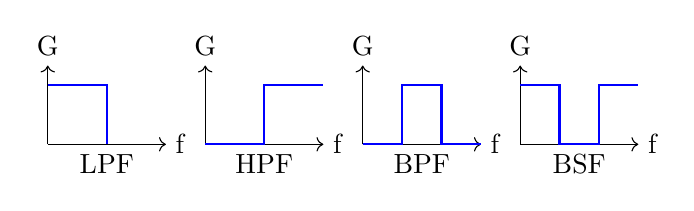
\begin{tikzpicture}[scale=0.5]
    % LPF
    \begin{scope}
    \draw[->] (0,0) -- (3,0) node[right] {f};
    \draw[->] (0,0) -- (0,2) node[above] {G};
    \draw[thick, blue] (0,1.5) -- (1.5,1.5) -- (1.5,0);
    \node at (1.5,-0.5) {LPF};
    \end{scope}
    
    % HPF
    \begin{scope}[xshift=4cm]
    \draw[->] (0,0) -- (3,0) node[right] {f};
    \draw[->] (0,0) -- (0,2) node[above] {G};
    \draw[thick, blue] (0,0) -- (1.5,0) -- (1.5,1.5) -- (3,1.5);
    \node at (1.5,-0.5) {HPF};
    \end{scope}
    
    % BPF
    \begin{scope}[xshift=8cm]
    \draw[->] (0,0) -- (3,0) node[right] {f};
    \draw[->] (0,0) -- (0,2) node[above] {G};
    \draw[thick, blue] (0,0) -- (1,0) -- (1,1.5) -- (2,1.5) -- (2,0) -- (3,0);
    \node at (1.5,-0.5) {BPF};
    \end{scope}
    
    % BSF
    \begin{scope}[xshift=12cm]
    \draw[->] (0,0) -- (3,0) node[right] {f};
    \draw[->] (0,0) -- (0,2) node[above] {G};
    \draw[thick, blue] (0,1.5) -- (1,1.5) -- (1,0) -- (2,0) -- (2,1.5) -- (3,1.5);
    \node at (1.5,-0.5) {BSF};
    \end{scope}
\end{tikzpicture}
\captionof{figure}{Ideal Frequency Responses}
\end{center}

\begin{mnemonicbox}
"LHBBA: Low High Band-pass Band-stop All-pass"
\end{mnemonicbox}
\end{solutionbox}

\section*{Question 5(c) OR [7 marks]}
\questionmarks{Question 5(c) OR}{7}{marks}

\textbf{Draw the circuit for T-section and $\pi$-section constant-K low pass filter and Derive equation of cut-off frequency.}

\begin{solutionbox}
\textbf{T-section Constant-K Low Pass Filter}:
\begin{center}
\begin{circuitikz}[american, scale=0.9]
    \draw (0,2) to[short, o-] (1,2) to[L, l=$L/2$] (3,2) coordinate(C) to[L, l=$L/2$] (5,2) to[short, -o] (6,2);
    \draw (C) to[C, l=$C$] (3,0) -- (3,0) coordinate(G);
    \draw (0,0) to[short, o-] (6,0) to[short, -o] (6,0);
\end{circuitikz}
\captionof{figure}{T-section LPF}
\end{center}

\textbf{$\pi$-section Constant-K Low Pass Filter}:
\begin{center}
\begin{circuitikz}[american, scale=0.9]
    \draw (0,2) to[short, o-] (1,2) to[short] (1,3) to[L, l=$L$] (5,3) to[short] (5,2) to[short, -o] (6,2);
    \draw (1,2) to[C, l=$C/2$] (1,0);
    \draw (5,2) to[C, l=$C/2$] (5,0);
    \draw (0,0) to[short, o-] (6,0) to[short, -o] (6,0);
\end{circuitikz}
\captionof{figure}{$\pi$-section LPF}
\end{center}

\textbf{Derivation of Cutoff Frequency}:
\begin{enumerate}
    \item For a constant-K filter:
    \begin{itemize}
        \item $Z_1 \times Z_2 = R_0^2$ (characteristic impedance squared)
        \item $Z_1 = j\omega L$ (series impedance)
        \item $Z_2 = \frac{1}{j\omega C}$ (shunt impedance)
    \end{itemize}
    \item $R_0^2 = j\omega L \times \frac{1}{j\omega C} = \frac{L}{C} \implies R_0 = \sqrt{L/C}$
    \item Pass band condition: $-1 < \frac{Z_1}{4Z_2} < 0$
    \item At cutoff frequency: $\frac{\omega^2 LC}{4} = 1$
    \item $\omega_c = \frac{2}{\sqrt{LC}}$
    \item $f_c = \frac{1}{\pi\sqrt{LC}}$
\end{enumerate}

\textbf{Final Equation}: $f_c = \frac{1}{\pi\sqrt{LC}}$

\begin{mnemonicbox}
"KCLP: Konstant-k Cutoff in Low Pass depends on L and C product"
\end{mnemonicbox}
\end{solutionbox}

\end{document}

